%2章
\chapter{提案手法}

本研究で対象とするエージェントシミュレーションの大きな特徴は,介護の対象となる高齢者の運動機能や認知機能の低下に大きなバリエーションがあると同時にも,介護者側にも国家資格をもった介護福祉士から,介護ヘルパー,ボランチィアスタッフまで技能や知識,経験に大きなバリエーションがあることである.そうしたことを念頭に置いた上で,本研究では介護者エージェント,被介護エージェント,環境としての高齢者施設の基本モデリングを検討した.図\ref{concept_simulation}に概念図を示す.黒で示される介護者が、自身が持つ視野の中で水色で示される被介護者を観測する.

\begin{figure}[htb]
\begin{center}
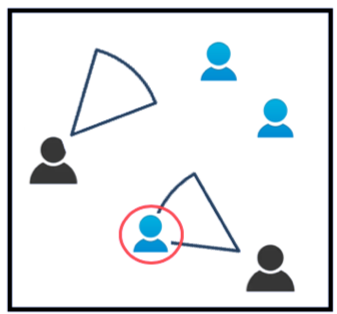
\includegraphics[scale=0.6]{figures/concept_simulation.png}
\caption[シミュレーションの概念図]{シミュレーションの概念図 \label{concept_simulation}}
\end{center}
\end{figure}

\section{知的マルチエージェントモデル}

介護行動は社会系の複雑現象である.私たちが行動を起こす際に,認知症による自己の生理機能への理解が周囲に与える影響を懸念することはあっても,それの繰り返しによって大きな事故につながると理解している人は少ない.しかし,個人レベルでは,手すりに捕まる,他の歩行者に接触しないようにするといった比較的単純なルールに従い行動しているが,それらの個人行動が多種・多量に存在し,相互作用することによって全体としては非常に複雑な現象となる.複雑系を解析する手法の一つとして,マルチエージェント手法がある.しばしば,セルオートマトンが複雑系のシミュレーションに用いられ,セルオートマトンに基づくシミュレーションの研究事例もいくつか存在する.これに対して,本シミュレータでは,人間という知的レベルの高い主体が多数集まり相互作用を起こす介護現象をより精緻に再現するために,情報を知覚し,それを基に自律的に行動を起こす主体を知的エージェント(IntelligentAgent),それを取り巻く世界を環境(Environment)と定義し,シミュレーションの構造はマルチエージェントのフレームワークに基づき構築している.そこで,これを知的マルチエージェントモデルと呼ぶ.

\subsection{知的エージェントの構築}
図\ref{intelligent_agent}に知的工一ジェントのイメージを示す.知的エージェントは,情報を知覚するセンサーと動作を実行する作用器を持っている.また,エージェント自身の思考プロセスを保持しており,センサーから得られた情報と自分の有する知識と判断基準に基づき自律的に行動を決定し,作用器を通して行動を起こし,環境に働きかける.センサー,作用器,思考は知的エージェントが実際に適用される時点で,問題に応じて定義される.図\ref{agent_modeling}にエージェントと環境の相互作用の様子を模式的に示す.介護者エージェントが自らの行動により環境に影響を与え、その環境によって被介護者エージェントが影響を受けることになる.ある主体の動きによって系全体の動きが規程され,複雑な現象が創発する.

\begin{figure}[htb]
\begin{center}
 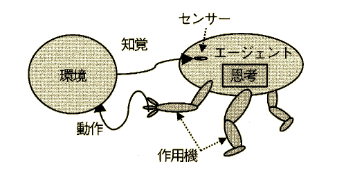
\includegraphics[scale=0.6]{figures/intelligent_agent.png}
 \caption[知的エージェントの模式図]{知的エージェントの模式図 \label{intelligent_agent}}
\end{center}
\end{figure}

\begin{figure}[htb]
\begin{center}
 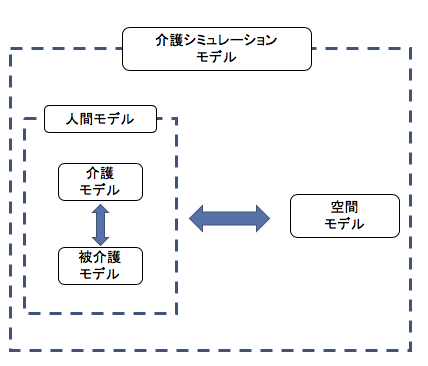
\includegraphics[scale=0.6]{figures/agent_modeling.png}
 \caption[本シミュレーションにおける環境とエージェント]{本シミュレーションにおける環境とエージェント \label{agent_modeling}}
\end{center}
\end{figure}

\subsection{Social force model}

本研究では,高齢者施設内で介護者が高齢者のトイレ介護のために空間移動するプロセスをモデリングするために,Socialforcemodel(SFM)\cite{SFM}という歩行者モデリング理論を用いる.SFMは,歩行者を2次元の粒子であると仮定し,その粒子に以下の4つの力が働くと仮定するモデルである.

\begin{itemize}
 \item 移動目標に近づく力
 \item 他のエージェントからの斥力
 \item 壁などの環境からの斥力
 \item 魅力的な環境への引力
\end{itemize}

移動目標に近づく引力は,エージェントが当初想定していたコースからはずれてしまった場合に目的地の進行方向へと曲げるように働く力のことであり,他のエージェントや壁などからの斥力は,エージェント間,あるいは壁とエージェント間との距離や,お互いの進行方向から決定される反発的な力のことである.魅力的な環境への引力では,友人やショーウィンドー,高齢者支援施設の中では手すりのような,歩行者にとって近づくことのインセンティブが発生するようなものへの引力のことである.これら4つの力は以下のように数式で表現される.

\begin{equation}
\begin{split}
 F_α(t)=F_α^o(υ_α,υ_α^0e_α)&+\sum_{β}F_αβ(e_α,r_α-r_β)\\
 &+\sum_{B}F_αβ(e_α,r_α-r_B^α)\\
 &+\sum_{i}F_αi(e_α,r_α-r_i,t)
\end{split}
\end{equation}

右辺第一項が移動目標に近づく力,第二項が他のエージェントからの斥力,第三項が壁などの環境からの斥力,第四項が魅力的な環境への引力を表している.各エージェントはタイムステップごとに以上の力を計算して,あらかじめ設定された最大歩行速度を超えないように歩行速度を更新する.

\subsection{介護ペア選択アルゴリズム}

MATESには,フランニング カ済んだ後に行う,1,」3抹示慨 産 を’丿.云 した.ただし,現 在のとこ ろプランニングー1乱 地,危.由地,目的地 など を定め る行為 )のブローヒスは 粕に入っていない.荊路探 索は,本来レ量と一身可能性の1斗 旦宏抱える雉しい問返であ る が.第1段階としてA*ア ルゴリズムIHに基づく経 路録才 滅能 を’メ装 した.さ ら に,探 索され た複Stの径路 力帚:・1つを丿一択するプロセスにつ  いては,−1   己に示 す オ1「路 選択に 圓わる複数の因子1a)出 発地か ら1=1的地 までの逗のり〔b:一尸E発 地か ら目的地 まで の旅 行 時 間「C)交デ厂』点で の直JL回叛(d:た」’:点で のノ折 回 数〔e>交差点で の右折 回 数〔1:1通 過す る道路の幅を9{:みつきて線形結合 し た)r’式の効1.1:II知数を定乳し,これ.亡 最 大にす る ものを /]二択す  る こ と と し た.

\section{仮想環境}
本シミュレータにおける環境とは,道路構造とそれに含まれる情報一般を指す.道路構造のモデル化はそれ自体が交通流シミュレータの汎用性・拡張性を実現する上で重要な課題である.本シミュレータでは,車は基本的に.申線(レーン)に沿って一次元制こ走行することを仮定する仮想走行レーンモデル101をベースとして道路モデルを構築しており,加えて仮想走行レーンモデルのみでは実現することが難しい大域的な経路探索や,車線変更,追い越し挙動などを実現するために,レーン束オブジェクトとレーン幅という概念を新たに導入した階層型道路モデルを構築した4).本研究では,これに加えて,歩行者を扱うために道路モデルを拡張した.

\subsection{高齢者施設}

現実には,車も歩行者も道路空間を移動するが,それぞれの移動範囲の時空間スケールや従うルールは大きく異なる場合も多い.こうした差異を無視して,道路環境に関して一元的な定義を彳∫うと,シミュレータの汎用性や拡張性を大きく損なうことになる.そこで,歩行者の存在空間を車の存在空問とは独立して定義し,歩彳亅.者空問と車空間のコミュニケーション方式を定義することにより,道路環境を定義することとした,また、今回の開発では,歩行者を扱うための第・ステップとして歩行者工一ジェントの存在範囲を横断歩道に限定した,これは,交通量の多い都市部の幹線道路においては,歩行者が自動車と相彑作用するのは交差点内の横断歩道がほとんどであると考えられるためである,歩行者は図3のような横断歩道エリアの中で行動する,横断歩道はそれぞれ固有の座標空間を持ち,2次元座標を川いてエージェントの位置を表す.横断歩道はエリアの境界に仮想的な滞留スペースを保持しており,歩行者は滞留スペースの中で絶えず発生している,歩行者の,横断歩道の幅方向の初期位骨はランダムに決定する.滞留スベースに存在する歩行者は,該当する信号が青である場合に横断歩道Eに登場する.

\subsection{介護者エージェント}

介護者工一ジェントは2次元の歩行者エリア上に存存するため,方向と速度の制御を行わなければならない.今回は,歩行者の行動モデルとしてSFMを採用した.また歩行者シミュレーションの研究分野において様々なモデル化が検剤されている\cite{ex_pedestrian_simulation_1,ex_pedestrian_simulation_2}.たとえば,磁気モデルを用いると多方向に歩行するエージェントの相互作用を効率的に記述することが可能である.しかし,今回の研究のように横断歩道上での歩行を対象とする場合には,単路を右から左,または左から右に渡る2方向を考慮すれば十分である,また歩行者モデルとしてあまり複雑なモデルを採用すると計算量が増大し交通シミュレータの大規模化が困難であることから,本研究では分岐型2ノ∫向モデルを採用した.以下で歩行者工一ジェントの特徴と挙動について述べる.\\
デルの単純化のために,人体を直径O.45m(成人男子の肩幅)の1[jで近似する.現バージョンのMATESでは高さの情報を解析に用いないため,平面で十分である,さらに,人体円の外側に他人の進入を拒む領域としてパーソナルスペースを設ける,パーソナルスペースとしては様々な形状が提案されているが\cite{ex_personal_space},本研究では1mの直径を持つ円をパーソナルスペースとして定めた.

\subsection{被介護者エージェント}

被介護者エージェントについては、介護者エージェントと同様にSocial Force Modelを軸に、歩行者エージェントを作成し、それに加えてエージェントの状態によって時系列的に発生する要介護行動を実装した.高齢者の排尿に関する実態研究 \cite{micturition} によると、排尿障害症状を自覚している人は男子が38%、女子が23%と高い水準にあり、男子では排尿困難症状が多く、女子では頻尿を訴える例が多かった。また明らかな尿失禁を抱えているのにも関わらず、その存在を知られたくないという心理が半数以上の人に認められたことも挙げられている。これらから、実際にトイレに行きたいと思っているかどうかの認知についてと、トイレで正常に排尿を行えるのかどうかといった機能について、被介護者のバリエーションを設けることとした.
